\documentclass[11pt]{article}
\usepackage[margin=0.78in]{geometry}
\usepackage[T1]{fontenc}
\usepackage{lmodern}
\usepackage{microtype}
\usepackage{graphicx}
\usepackage{booktabs}
\usepackage{tabularx}
\usepackage{longtable}
\usepackage{array}
\usepackage{amsmath}
\usepackage{xcolor}
\usepackage{enumitem}
\usepackage{xurl}
\usepackage{hyperref}
\usepackage{caption}
\hypersetup{colorlinks=true,linkcolor=blue!55!black,urlcolor=blue!55!black,citecolor=blue!55!black}
% Keep figures inside the paper project so the built-in editor can bundle them.
\graphicspath{{figures/}}
\setlength{\parskip}{0.42em}
\setlength{\parindent}{0pt}
\setlength{\emergencystretch}{1em}
\renewcommand{\arraystretch}{1.18}
\captionsetup{font=small,labelfont=bf}
\newcommand{\pp}{\,\mathrm{pp}}
\newcommand{\ci}[2]{[#1,\,#2]}

\title{Windowed Execution Fingerprints for Human/Agent Trace Analysis\\\large Method, Data, and Exploratory Results}
\author{AttackAgent Detect research notes}
\date{2 November 2026}

\begin{document}
\maketitle

\begin{abstract}
We test whether a compact, interpretable matrix of command and coarse-action statistics can describe execution traces, distinguish released Human/Agent labels, and help retrieve same-task traces. The matrix contains eight measurements per variable-length command window. On 89 eligible AIT troubleshooting runs, its 24-value window summary reaches 56.3\% task-macro balanced accuracy (BA), versus 55.2\% for a whole-session eight-feature summary; the paired difference is only +1.1 percentage points (95\% task-bootstrap interval $[-14.3,+15.4]$). Command TF--IDF reaches 96.8\%, while the matrix falls to 39.9\% under source-group holdout, exposing a strong collection/label dependence. Across target Agent-role shares from 0\% to 100\% in 17 Cyber Task Horizons (CTH) challenges, task-macro BA falls from 53.8\% to 46.0\% for command cosine (paired change $-7.7$ pp, 95\% task-cluster interval $[-16.0,-0.4]$) and from 57.3\% to 46.0\% for action-bigram cosine ($-11.3$ pp, $[-20.8,-3.3]$). FMR falls while FSR rises, indicating a shift toward missed same-task retrieval under the fixed threshold. The matrix adds 0.35 pp to CTH Agent-only Hit@1 and 2.08 pp to Antieval Cybench Hit@1; both paired intervals include zero. These are exploratory, source-qualified benchmark results. Shared challenge identity is a task-retrieval proxy, not a shared operator, attack, or campaign label.
\end{abstract}

\section{Question and scope}
Behavioral trace association commonly uses trace similarity as association evidence, for example through tool use, operation order, or system-behavior sequences. We investigate whether Human versus Agent execution changes this similarity and the resulting same-task association decisions. Agent-mediated execution can introduce model, framework, prompt, and tool-configuration influences alongside the task and environment; these influences could affect the meaning of observed similarity without necessarily making traces more alike or less alike.

We construct a multidimensional behavioral fingerprint from common logs, turning tool use, action organization, and local repetition into comparable evidence. The broader research objective is to investigate whether this representation can support trace retrieval across execution modes, investigation triage, and evidence-proportionate association confidence. The present study operationalizes this objective through label recognition and benchmark task retrieval; downstream investigative value and calibrated confidence remain research goals, not demonstrated outcomes.

We separate three questions: (1) can the measurements predict the released Human/Agent labels in a held-out task? (2) how do a same-challenge retrieval baseline's errors vary as the Human/Agent composition of query--candidate roles changes? (3) does adding the fingerprint improve source-local Agent-only task retrieval? The first question uses AIT audit logs, while the latter two use CTF/tool-call datasets. Their labels and metrics are not pooled.

\section{Data and relation labels}
The registry contains 1,142 normalized records: 664 CTF and 478 supplemental task/security traces. Each analysis below uses only its qualified subset.

\begin{table}[ht]
\centering
\small
\caption{Separate experimental tracks. Counts refer to eligible observations, not the full source releases.}
\begin{tabularx}{\linewidth}{@{}p{0.17\linewidth}p{0.24\linewidth}p{0.22\linewidth}X@{}}
\toprule
Track & Data and eligible size & Label or relation & Intended inference \\
\midrule
Mode recognition & AIT shell troubleshooting: 89 runs, 45 Human / 44 Agent, 12 task groups & Released execution-mode label & Predict labels on held-out task/source/application groups; the label remains entangled with collection and workflow \\
Mixture retrieval & CTH CTF: 17 challenge groups, 85 records in selected groups & Same source-qualified challenge vs. a different challenge & Compare FMR/FSR and ranking across controlled Human/Agent role mixtures \\
Agent-only retrieval & CTH: 121 traces / 48 tasks; Antieval Cybench: 31 / 12 tasks & Same source-qualified task within each source & Test whether matrix features change same-task Hit@1 within source \\
\bottomrule
\end{tabularx}
\end{table}

The archived AIT release contains 109 raw run logs; 95 parsed common-view runs were available in the prior pilot and 89 pass this matrix study's evidence gate. AIT tasks are Nextcloud/WordPress troubleshooting, not attacks. CTH Human records are terminal recordings and Agent records are structured tool calls. Antieval Cybench contributes Agent-only HTTP/tool trajectories. These are different observation contracts. A shared CTF challenge identifies a common task context only; it is not ground truth for a common actor, Agent instance, attack activity, host, organization, or campaign.

An additional Human-only task supplement has now been ingested from the KYPO Locust training release~\cite{kypo}: 100 participants yield 359 participant--level segments, of which 265 have a nonempty common shell-command view. Ten source/variant/level task groups contain repeated Human traces. At a minimum of eight retained commands, 146 segments remain (145 in nine tasks with at least two Humans), versus 68 segments at sixteen commands (67 in seven repeated tasks). These are dependent segments from 100 participants, not 359 independent people. No matched Agent runs are available for these tasks, so this supplement contributes Human--Human task evidence and has not been included in the Human/Agent recognition or mixture scores reported here. Data1 and data2 retain separate task namespaces.

\section{Fingerprint method}
We use the ordered executable/tool names exposed by each source adapter and map recognized commands to eight coarse action groups: discover, read, search, execute, build, network, modify, and environment. These are lossy observable traces; they do not expose an Agent's internal reasoning. We exclude IDs, task/source labels, model names, prompts, paths, timestamps, and capture-format strings from features.

For command window $w=(c_1,\ldots,c_n)$, let $p(c)$ be the empirical command-name distribution and let $a_i$ be the mapped coarse action when available. The feature vector $\mathbf{k}_w=(K_1,\ldots,K_8)$ is:
\begin{align*}
K_1&=|\{c_i\}|/n, & K_2&=-\sum_c p(c)\log_2 p(c), & K_3&=\max_c p(c),\\
K_4&=\Pr(a_i\ne a_{i+1}), & K_5&=H(A_{i+1}\mid A_i), & K_6&=L_{\max}(a)/n,\\
K_7&=1-|\{(a_i,a_{i+1})\}|/|P_a|, & K_8&=\Pr(c_i=c_{i+1}).
\end{align*}
Here $P_a$ contains adjacent pairs whose two action labels are known; $L_{\max}$ is the longest consecutive run of one mapped action. A statistic with insufficient mapped observations is missing, not zero.

Commands are partitioned into consecutive windows of eight. The matrix has a variable number of rows, $J\times8$: at least 16 commands are required, at most the first 128 are used, and a final tail shorter than four commands is discarded. We do not impose a fixed number of attack phases. For the classifier, each column is summarized by its mean, population standard deviation, and least-squares slope over normalized window position, yielding 24 values. Missing values are imputed from training data only, then standardized and passed to class-balanced logistic regression ($C=1$, threshold 0.5). The direct sequence matcher uses masked dynamic time warping (DTW) over train-scaled columns; a local cost requires at least three shared finite columns.

\begin{table}[ht]
\centering
\small
\caption{The eight fingerprint dimensions. The definitions are operational measurements, not claims that a feature is unique to an Agent.}
\begin{tabularx}{\linewidth}{@{}c p{0.25\linewidth}X@{}}
\toprule
ID & Dimension & Window-level measurement \\
\midrule
K1 & Executable diversity & Distinct command names divided by command count \\
K2 & Command entropy & Shannon entropy (bits) of command-name frequencies \\
K3 & Dominant command share & Frequency of the most common command name \\
K4 & Action switching & Fraction of mapped adjacent action pairs that change group \\
K5 & Transition uncertainty & Conditional entropy of the next mapped action given the current action \\
K6 & Longest action run & Longest consecutive run of one mapped action, divided by window length \\
K7 & Repeated action-pair share & One minus the fraction of unique mapped adjacent action pairs \\
K8 & Repeated command adjacency & Fraction of adjacent commands with identical names \\
\bottomrule
\end{tabularx}
\end{table}

\begin{figure}[ht]
\centering
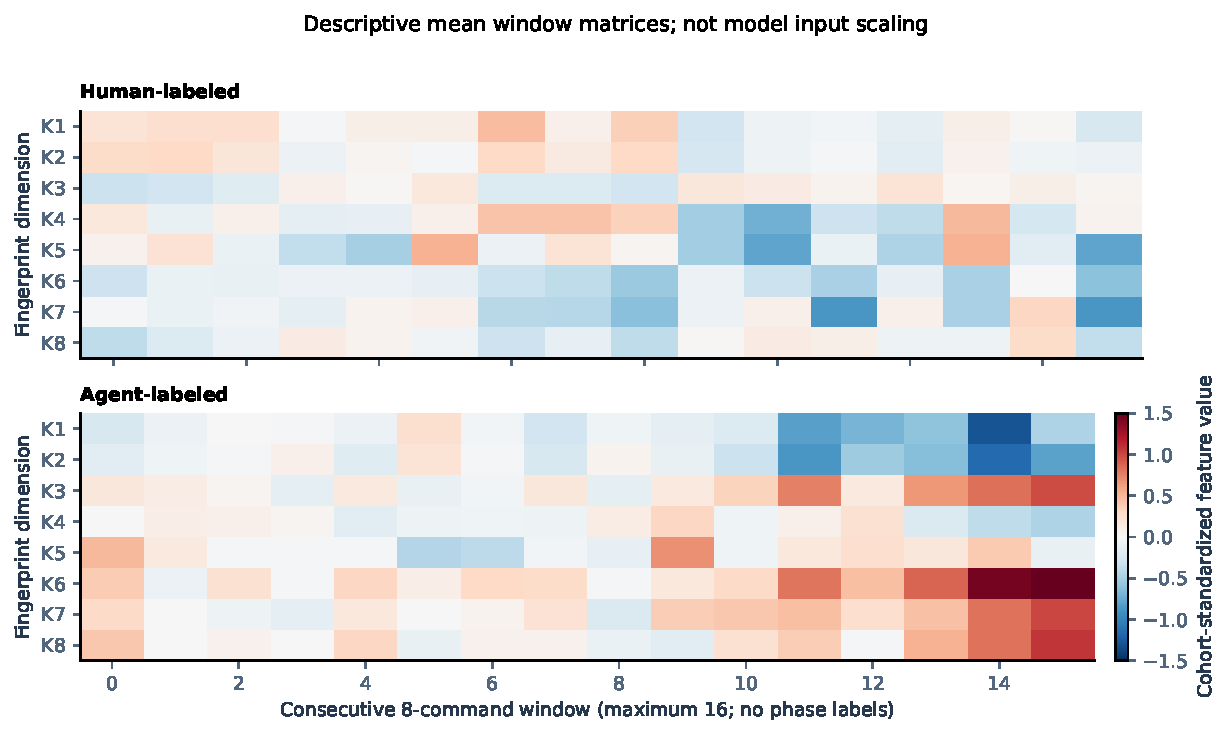
\includegraphics[width=.88\linewidth]{ait-window-fingerprint-matrix.pdf}
\caption{Observed AIT matrix example summarized by cohort for visualization. Each row is one eight-command window and each column one of K1--K8. Values are cohort-standardized for display; this figure is not a learned classifier and does not imply a universal Agent profile.}
\end{figure}

\section{Experimental protocol}
\subsection{Human/Agent label recognition}
The primary AIT split holds out task groups; exact duplicate command sequences are purged across train and test. Secondary panels hold out source groups, application, or both task and source. We compare command-count length, command-name unigram/bigram TF--IDF, whole-session K1--K8, the 24-value window summary, and matrix-DTW 3-nearest-neighbor. Classifier hyperparameters are fixed; there is no score-based feature or window selection. We report task-macro BA and task-cluster bootstrap intervals over fixed out-of-fold predictions. These intervals do not include retraining uncertainty.

\subsection{CTF mixture and pair-type errors}
The CTH cohort has 17 tasks with at least two Human and two Agent sessions each. For each held-out query we rank five candidates: one same-task positive and four different-task negatives. We assign Human/Agent roles to target Agent shares of 0\%, 25\%, 50\%, 75\%, and 100\%, with 100 repeated draws per level. Because the 17 tasks provide 34 query/gallery role slots, integer allocation realizes the 25\% and 75\% targets as 8/34 (23.5\%) and 26/34 (76.5\%); plots and tables label the prespecified target levels. Repeated draws are not independent samples. We compare command TF--IDF cosine and coarse action-bigram cosine. A threshold is selected using task-cross-fitted training pairs only: maximize positive recall subject to training negative FMR $\leq10\%$. We report FMR, FSR, task-macro BA $=1-(\mathrm{FMR}+\mathrm{FSR})/2$, and Hit@1. BA uncertainty and endpoint contrasts use a paired task-cluster bootstrap after averaging each task over the 100 role draws. Pair types HH, HA, and AA are calculated from query/candidate execution labels, not as separate concentration experiments.

The matrix-mixture increment was not run: only one task has at least two Human and two Agent sessions with 16 or more commands, below the predeclared minimum of 15 such tasks. Therefore this experiment cannot test whether the matrix repairs Human/Agent mixture errors.

\subsection{Agent-only task retrieval}
For each source separately, tasks are split into three fixed folds before candidate formation. Each query has one same-source-task positive and either four (CTH) or two (Antieval) different-task candidates. We compare command cosine with a fixed logistic fusion of command cosine and negative masked-DTW distance, trained on training-task pairs. The primary metric is task-macro Hit@1; uncertainty is a task-cluster bootstrap. Cross-source direction tests train on one source and evaluate source-native retrieval in the other; no cross-source challenge identity is assumed. These transfer runs are post-observation exploratory because both sources were used for protocol development.

\section{Results}
\subsection{The matrix is measurable, but label recognition is dominated by source-visible command vocabulary}
On the primary held-out-task panel, command TF--IDF reaches 96.8\% task-macro BA, while the matrix summary reaches 56.3\% (95\% CI [40.8,71.7]) and the whole-session K1--K8 baseline reaches 55.2\% (95\% CI [46.1,65.9]). The paired window-minus-whole-session difference is +1.1 pp (95\% task-bootstrap interval $[-14.3,+15.4]$, 12 tasks). Matrix DTW 3-NN reaches 53.3\%. The lexical result is a strong predictor of these released labels, but the Human/Agent collection pathway and operating workflow are not experimentally separated, so it is not an isolated actor-identity result.

\begin{table}[ht]
\centering
\small
\caption{Primary AIT task-held-out results. The 95\% intervals are task-cluster intervals on fixed out-of-fold predictions.}
\begin{tabular}{@{}l r r l@{}}
\toprule
Model & Task-macro BA & Macro-F1 & 95\% BA interval \\
\midrule
Length only & 46.6\% & 51.7\% & [32.6,59.7] \\
Command TF--IDF & 96.8\% & 95.5\% & [94.2,99.2] \\
Whole-session K1--K8 & 55.2\% & 55.0\% & [46.1,65.9] \\
Window summary & 56.3\% & 57.3\% & [40.8,71.7] \\
Matrix DTW 3-NN & 53.3\% & 56.0\% & [46.4,60.1] \\
\bottomrule
\end{tabular}
\end{table}

\begin{table}[ht]
\centering
\small
\caption{Task-macro BA across held-out panels. These secondary panels use the same frozen 89-run cohort.}
\begin{tabular}{@{}l r r r r@{}}
\toprule
Model & Task & Source group & Application & Task + source \\
\midrule
Command TF--IDF & 96.8\% & 82.6\% & 95.1\% & 80.0\% \\
Window summary & 56.3\% & 39.9\% & 45.8\% & 37.6\% \\
Matrix DTW 3-NN & 53.3\% & 36.9\% & 50.8\% & 37.8\% \\
\bottomrule
\end{tabular}
\end{table}

The secondary holdouts show that the feature representation does not carry a stable execution-mode signal across these collection groups. Command TF--IDF remains predictive, but it too falls under stronger source/task controls. This pattern is consistent with vocabulary, workflow, and instrumentation carrying substantial information; it does not show that K1--K8 are an Agent-specific signature.

\begin{figure}[ht]
\centering
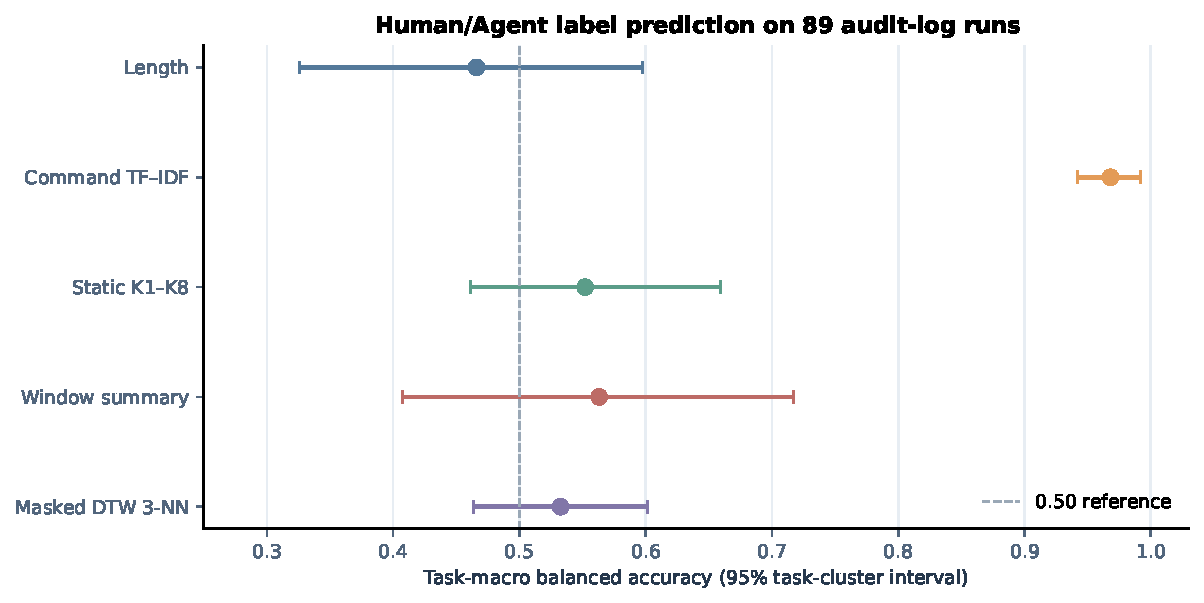
\includegraphics[width=.93\linewidth]{ait-recognition-task-holdout.pdf}
\caption{AIT held-out-task classifier comparison. Error bars are task-cluster bootstrap intervals on fixed predictions.}
\end{figure}

\begin{figure}[ht]
\centering
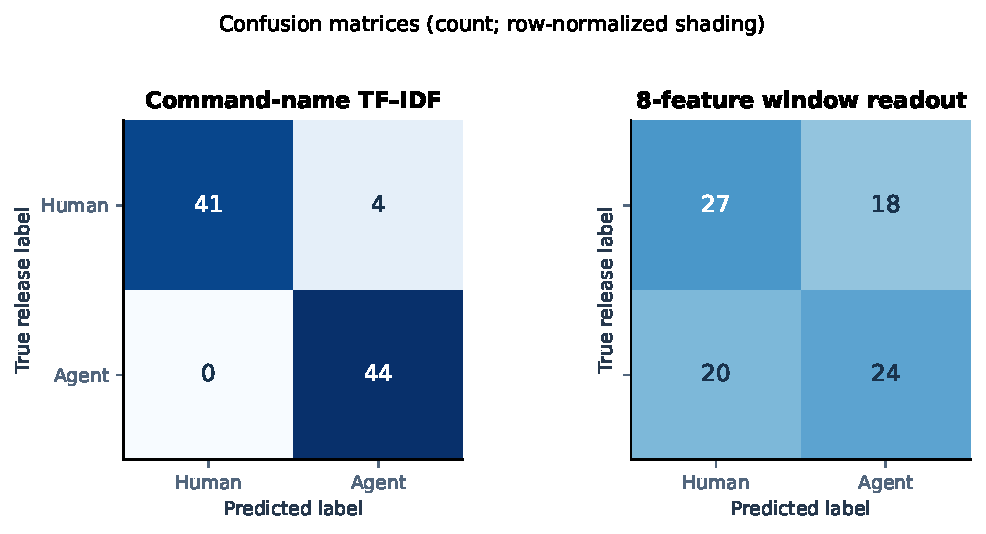
\includegraphics[width=.58\linewidth]{ait-recognition-confusion.pdf}
\caption{Fixed-threshold confusion matrices for command TF--IDF and the window-summary classifier on held-out tasks. Rows are released Human/Agent labels; columns are predicted labels.}
\end{figure}

\subsection{Agent mixture shifts the observed error from merging toward splitting}
For command cosine, moving from 0\% to 100\% target Agent roles changes FMR from 27.8\% to 9.6\%, while FSR changes from 64.7\% to 98.4\%. The composite task-macro BA falls from 53.8\% to 46.0\%, a paired change of $-7.7$ percentage points (95\% task-cluster interval $[-16.0,-0.4]$, 17 tasks). Action-bigram cosine shows the same pattern: FMR 32.4\% to 9.6\%, FSR 52.9\% to 98.4\%, and BA 57.3\% to 46.0\% (paired change $-11.3$ pp, 95\% interval $[-20.8,-3.3]$). The aggregate result therefore indicates worse thresholded same-task retrieval in this CTF proxy setting as the target Agent share rises, while the error composition shifts from false merges toward false splits. It does not support the preregistered directional story that increasing Agent concentration raises false merges. Hit@1 rankings and thresholded links are different measurements.

\begin{table}[ht]
\centering
\small
\caption{CTH command-cosine results by target Agent role share. FMR/FSR are thresholded link errors; Hit@1 is rank-based. Task-macro BA is $1-(\mathrm{FMR}+\mathrm{FSR})/2$.}
\begin{tabular}{@{}r r r r r@{}}
\toprule
Target Agent share & FMR & FSR & Task BA & Hit@1 \\
\midrule
0\% & 27.8\% & 64.7\% & 53.8\% & 41.5\% \\
25\% & 20.2\% & 77.0\% & 51.4\% & 36.5\% \\
50\% & 11.8\% & 88.1\% & 50.1\% & 35.1\% \\
75\% & 7.8\% & 96.4\% & 47.9\% & 34.9\% \\
100\% & 9.6\% & 98.4\% & 46.0\% & 39.1\% \\
\bottomrule
\end{tabular}
\end{table}

The table and figure use the target mixture labels. Integer role allocation yields realized Agent shares of 23.5\% and 76.5\% at the 25\% and 75\% targets, respectively.

At the 50\% level, the command baseline's pair-type estimates are HH: FSR 64.7\% / FMR 28.2\%; HA: 93.6\% / 5.9\%; AA: 98.6\% / 9.7\%. The dominant observed issue is missed same-task retrieval for mixed-mode and Agent--Agent positives under this operating threshold. Since these are CTF task proxies and the capture interfaces differ, we cannot conclude that this is real attack-activity fragmentation.

\begin{figure}[ht]
\centering
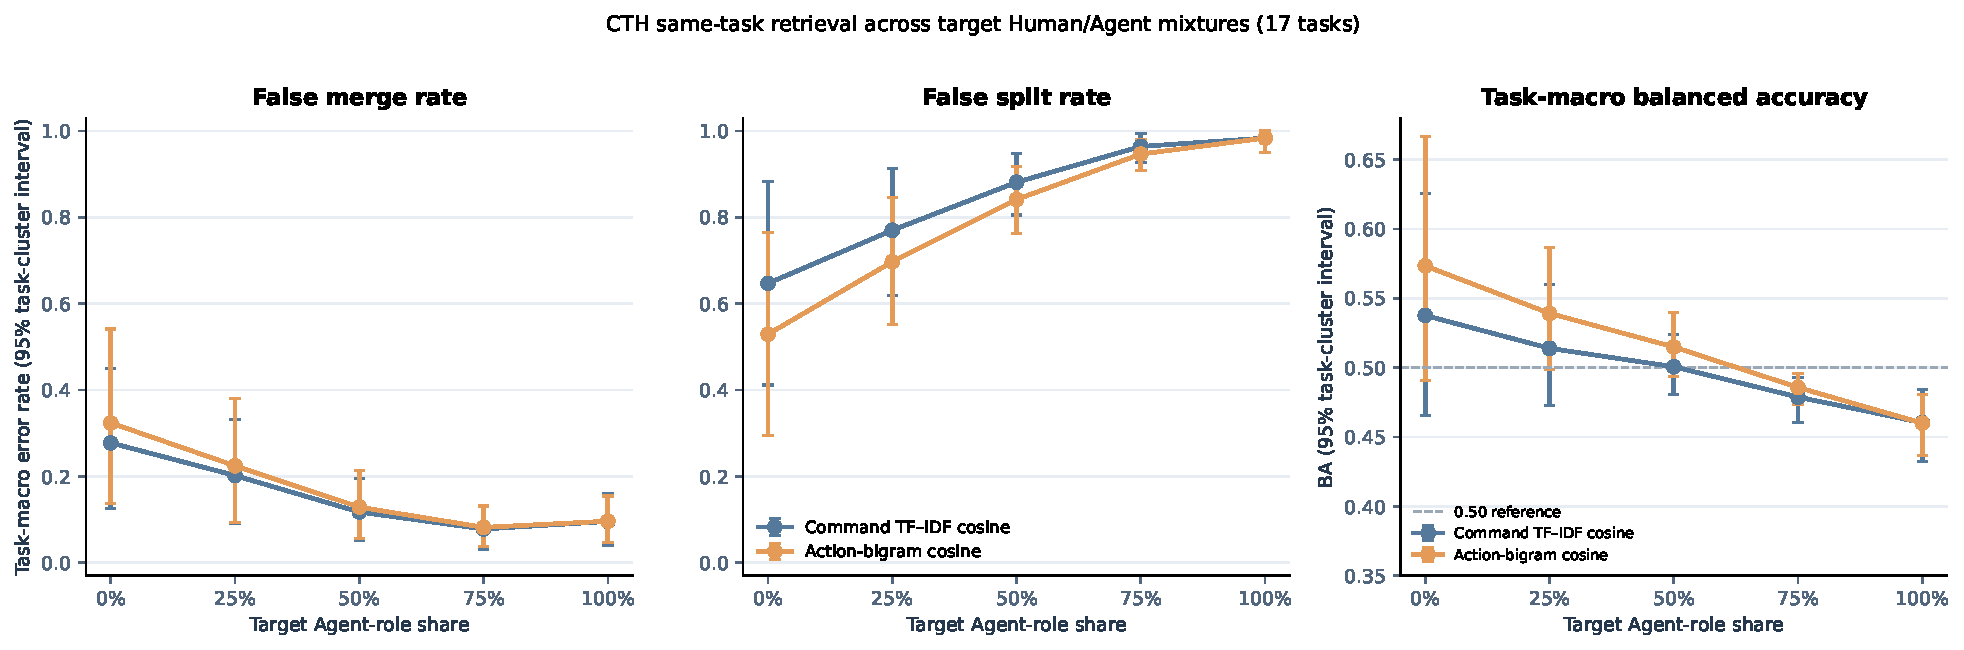
\includegraphics[width=\linewidth]{ctf-mixture-errors.pdf}
\caption{Three-panel CTH mixture results: false-merge rate, false-split rate, and composite task-macro balanced accuracy for command and action-bigram cosine. The x-axis shows target Agent-role shares; the 25\% and 75\% targets realize as 23.5\% and 76.5\% under integer role allocation. Points summarize 100 repeated draws; 95\% intervals resample the 17 task clusters after averaging within task, not the repeated draws as independent samples.}
\label{fig:ctf-mixture-composite}
\end{figure}

\begin{figure}[ht]
\centering
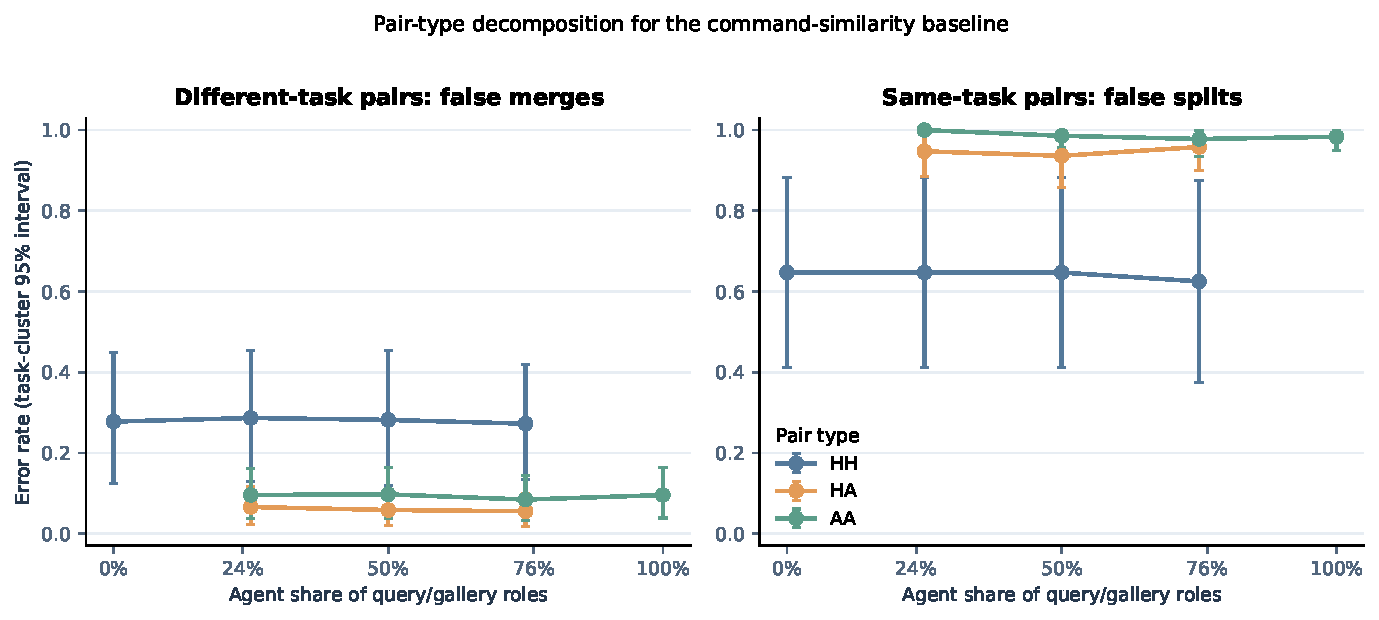
\includegraphics[width=.92\linewidth]{ctf-pair-type-errors.pdf}
\caption{CTH error rates separated by HH, HA, and AA query--candidate pairs. A pair type is a composition of two execution labels, while Agent concentration is a cohort-level role allocation.}
\end{figure}

\subsection{Adding the matrix does not reliably improve Agent-only retrieval}
In CTH, command-cosine Hit@1 is 54.9\% (five candidates; chance 20\%) and matrix fusion is 55.2\%, a paired gain of +0.35 pp (95\% task-bootstrap interval $[-3.82,+4.17]$, 48 tasks). In Antieval Cybench, the corresponding values are 60.4\% and 62.5\% (three candidates; chance 33.3\%), a +2.08 pp change (95\% interval $[-6.25,+12.50]$, 12 tasks). These uncertain task-retrieval results do not validate the matrix as an association correction.

\begin{table}[ht]
\centering
\small
\caption{Source-local Agent-only retrieval and paired change after matrix fusion. Candidate counts differ, so rows must not be pooled.}
\begin{tabular}{@{}l r r r r@{}}
\toprule
Source & Queries / tasks & Command Hit@1 & Fused Hit@1 & Paired change (95\% CI) \\
\midrule
CTH & 121 / 48 & 54.9\% & 55.2\% & +0.35 pp $[-3.82,+4.17]$ \\
Antieval Cybench & 31 / 12 & 60.4\% & 62.5\% & +2.08 pp $[-6.25,+12.50]$ \\
\bottomrule
\end{tabular}
\end{table}

\begin{figure}[ht]
\centering
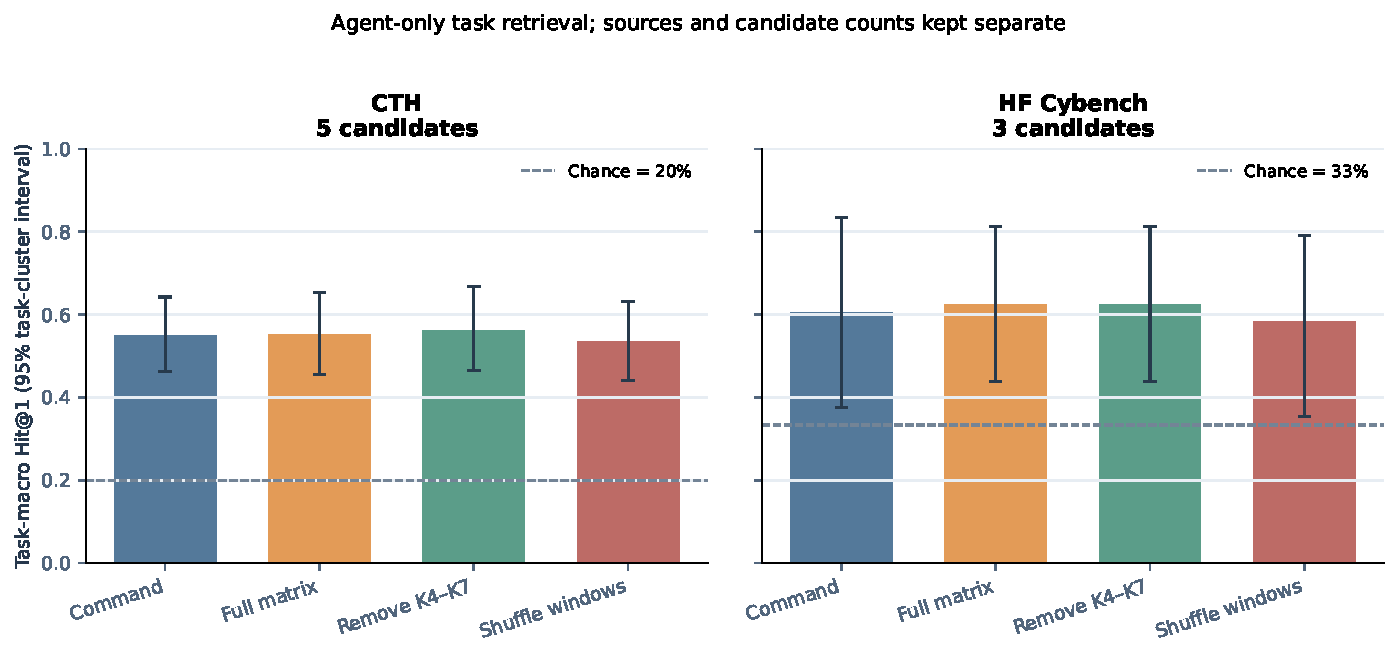
\includegraphics[width=.85\linewidth]{agent-retrieval-ablation.pdf}
\caption{Paired task-macro Hit@1 differences for matrix fusion and feature-group ablations, kept separate by source. The candidate sets are source-specific.}
\end{figure}

\subsection{Small Human-to-Agent same-challenge probe: exploratory}
A subsequent fixed probe joins CTH Human queries to an Antieval Agent gallery using normalized CyBench challenge slugs. All five overlapping IDs are retained: back\_to\_the\_past, flag\_command, locktalk, lootstash, and packedaway. Seven Human traces and 30 Agent traces have at least four retained commands; this relaxed gate and four-command windows belong to this probe only. Each Human query ranks one same-challenge Agent candidate and one negative from each of the other four challenges, with 20 common gallery draws per query. For each held-out query challenge, scaling and fusion are fitted on Agent-only pairs from the other four challenges, without tuning on the query challenge.

Task-macro Hit@1 is 44.0\% for command cosine and 42.5\% for command plus matrix-DTW, a paired change of $-1.5$ pp (95\% task-cluster interval $[-4.5,0.0]$; five clusters, 10,000 resamples). MRR changes from 0.681 to 0.671 and pairwise AUC from 0.784 to 0.776. The command-plus-length control reaches 39.0\% Hit@1. This probe provides no positive matrix increment. Its 20 repeated draws per query are averaged within task and do not enlarge the five independent challenge clusters. Challenge slugs are a provisional cross-source task proxy: fixture/version equivalence and capture parity remain unverified. These scores are exploratory and are not a replacement for the frozen mixed-mode experiment that failed its evidence gate.

\section{Relation to prior work}
Trace studies command-sequence classification for underlying model-family inference~\cite{trace}, and ProcGrep studies procedural traces for coding-agent identification~\cite{procgrep}; both motivate behavioral measurement but use different labels and domains. ATLAS and HOLMES use system-behavior evidence to reconstruct or associate attack stories~\cite{atlas,holmes}, but they do not identify Human versus Agent execution. Synthetic APT experiments motivate testing whether Agent-mediated behavior changes attribution cues~\cite{synthetic}; they do not provide evidence for the outcomes in this study. Our CTF task-match evaluation is a deliberately narrower proxy, not a reproduction of campaign attribution. Source diversity is a design direction for broadly usable trace tools, but the present small transfer experiment does not demonstrate broad generalization.

\section{Limitations and next measurement}
The association findings are limited to same-task retrieval and pairwise matching under the public benchmark labels and candidate sets used here. The available data do not provide independently verified links for real attack activities, campaigns, or common operators, and do not hold logging, environment, and execution system constant across all Human/Agent comparisons. We therefore cannot yet validate the proposed fingerprint for those broader association relations, claim causal degradation from Agent participation, or establish improved operational association confidence. Even a confirmed same-task gain would require separate validation before supporting those conclusions.

The AIT Human/Agent label is coupled to model/person groups and their software-task workflow. CTH also couples label to terminal-versus-tool-call capture. The CTF positive label is same benchmark challenge, and the tested logs omit much internal Agent state. Small task counts produce wide uncertainty. Repeated mixture draws refine sampling estimates within these 17 tasks but do not create new independent tasks. Cross-source transfer is exploratory, and the matrix increment for mixed Human/Agent retrieval was blocked by the frozen evidence gate.

The next high-value dataset is a matched logging collection: the same command/action schema, task, permissions, and environment recorded under Human and Agent execution, with repeated runs and model/framework/prompt configuration retained as audit metadata but withheld from the classifier. Longer paired traces would make the matrix-mixture test eligible. This would distinguish execution-mode evidence from instrumentation and task vocabulary more directly.

\appendix
\section{Complete mixture results}
\begin{table}[ht]
\centering
\small
\caption{CTH action-bigram cosine across Agent role mixtures.}
\begin{tabular}{@{}r r r r r@{}}
\toprule
Target Agent share & FMR & FSR & Task BA & Hit@1 \\
\midrule
0\% & 32.4\% & 52.9\% & 57.3\% & 38.9\% \\
25\% & 22.5\% & 69.7\% & 53.9\% & 34.3\% \\
50\% & 12.9\% & 84.1\% & 51.5\% & 32.1\% \\
75\% & 8.2\% & 94.7\% & 48.6\% & 28.6\% \\
100\% & 9.6\% & 98.4\% & 46.0\% & 26.3\% \\
\bottomrule
\end{tabular}
\end{table}

At the 50\% mixture, command-cosine pair-type 95\% task-cluster intervals are: HH FSR [41.2,88.2]\%, FMR [11.8,45.5]\%; HA FSR [85.7,100.0]\%, FMR [2.0,10.3]\%; AA FSR [95.7,100.0]\%, FMR [3.8,16.4]\%. These are descriptive intervals across the 17 task groups.

\section{Recognition ablations and controls}
On the primary held-out-task predictions, removing K1--K3 changes task-macro BA by +5.0 pp (95\% paired task-bootstrap interval $[0.0,+11.5]$); removing K4--K7 changes it by $-5.5$ pp $[-18.0,+7.7]$; removing K8 changes it by $-2.3$ pp $[-11.7,+4.0]$. The evidence does not isolate a stable winning feature group. Shuffling window order does not establish a robust ordered-sequence contribution. The fixed-first-32 comparison is restricted to 47 runs across seven tasks, so it is not directly comparable to the 89-run primary cohort.

\section{Cross-source retrieval: exploratory}
\begin{table}[ht]
\centering
\small
\caption{Train in one source; rank target-source-native same-task candidates in the other. No task identities are linked across sources.}
\begin{tabular}{@{}l l r r r r@{}}
\toprule
Train & Test & Test tasks / queries & Command Hit@1 & Fused Hit@1 & Paired change (95\% CI) \\
\midrule
CTH & Antieval & 12 / 31 & 51.4\% & 51.4\% & 0.00 pp [0.00,0.00] \\
Antieval & CTH & 48 / 121 & 52.8\% & 54.5\% & +1.74 pp $[-3.82,+6.94]$ \\
\bottomrule
\end{tabular}
\end{table}

\begin{figure}[ht]
\centering
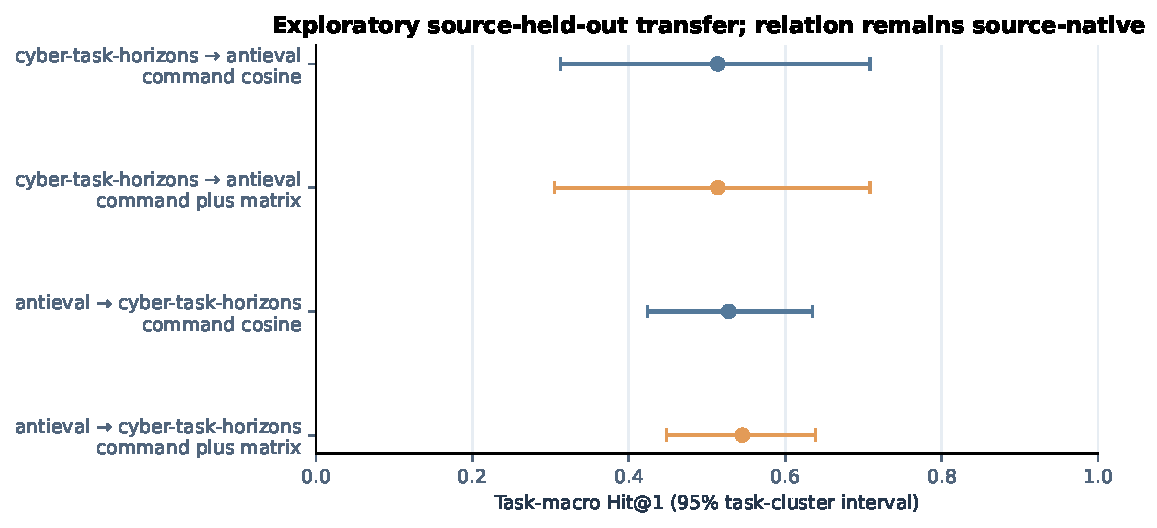
\includegraphics[width=.83\linewidth]{agent-retrieval-cross-source.pdf}
\caption{Exploratory transfer scores. Chance differs because candidate counts are three and five. The zero observed gain in CTH-to-Antieval is based on 12 test tasks and should not be read as proof of equivalence.}
\end{figure}

\section{Planned next study: sequence and real-time execution rhythm}
This is a prospective design, not an additional result. The next primary evaluation must use newly collected Human/Agent sessions under a common logging contract. Existing catalog records and repeated splits of the old cohorts do not constitute new data. The proposed collection uses resettable, version-pinned tasks, common host-side launch and exit events, relative monotonic timestamps, execution outcomes, and process ancestry for both modes. Actual Human participants supply Human labels; generated demonstrations cannot substitute for them.

The candidate fingerprint retains the eight local measurements and adds eight sequential-context measurements (tool novelty, nonadjacent revisits, return spans, lagged action returns, command-fragment reuse, and adjacent-window distribution change) and eight timing measurements (log-gap median and IQR, burstiness, fractions of gaps at most 1 second or at least 10 seconds, lag-1 gap correlation, matched execution duration, and completion-to-next-start idle time). The complete candidate has shape $J\times24$ with explicit missingness; its three blocks are feature families, not fixed attack phases. Mean/SD/slope readout yields 72 classification values. Launch gaps, program runtime, and idle time remain distinct observations; gaps are not automatically interpreted as thinking time.

The initial collection target is six pilot tasks (48 new runs), followed by 24 different formal tasks split 12/6/6 into training/validation/test (192 new runs). Each task targets two actual Human sessions and two repeats for each of three recorded Agent configurations. Formal Human participant groups are disjoint across splits. These are planning targets, not collected samples or a power guarantee. Pilot variance and resource constraints determine any pre-collection adjustment; the sealed test is not repeatedly inspected for feature selection.

The primary recognition endpoint is held-out-task macro BA. The primary association endpoint is paired task-macro BA gain over command cosine at a 50\% target Agent share, with the threshold frozen before test evaluation. Secondary panels report 0/25/50/75/100\% target shares, actual integer allocation, HH/HA/AA errors, ranking, coverage, and calibration. Ablations remove sequence or time blocks, permute command positions or time-gap order, and control command count and runtime. Repeated windows and candidate draws are not independent tasks. New data would strengthen matched task-level evidence; real activity, campaign, and common-operator association would still require their own validated relation labels.

The full prospective plan, candidate definitions, and collection-slot allocation are in \url{research/experiments/temporal_fingerprint_v2/}. Experimental-design workflow assistance used Scientific Agent Skills~\cite{skills}; that software reference is not evidence for fingerprint effectiveness.

\section{Reproduction and artifacts}
The run used the frozen protocol and fixed seed 20261102. Original task-cluster intervals use 2,000 bootstrap resamples; the added composite mixture BA intervals and paired endpoint contrasts use 20,000 task-cluster resamples, recorded in \url{mixture/composite-balance.json}. The final runner completed recognition, mixture, and both Agent-only retrieval directions. Early runner failures were cohort/fold bookkeeping errors and are retained in the run ledger; they are not experimental outcomes. Reproduce from the repository root:
\begin{verbatim}
.venv/bin/python research/experiments/overnight_fingerprint_v1/run.py all
.venv/bin/python research/experiments/overnight_fingerprint_v1/build_figures.py
\end{verbatim}
Full predictions, fold assignments, eligibility lists, metrics, and hashes are in \url{research/results/overnight_fingerprint_v1/}. The associated research and source notes are \url{site/local-mode-detector.html#results} and \url{site/related-work.html#round-results}.

The subsequent Human-to-Agent same-challenge probe has a separate fixed exploratory program and results under \url{research/experiments/matched_human_agent_probe_v1/} and \url{research/results/matched_human_agent_probe_v1/}; its task-cluster intervals use 10,000 resamples. It is reproduced with \texttt{.venv/bin/python research/experiments/matched\_human\_agent\_probe\_v1/run.py}.

\begin{thebibliography}{99}\small
\bibitem{ait} AIT/AECID, \emph{LLM User Shell Simulation}, source and audit-log release. \url{https://github.com/ait-aecid/llm-user-shell-sim}.
\bibitem{cth} Lyptus Research, \emph{Cyber Task Horizons data}. \url{https://github.com/lyptus-research/cyber-task-horizons-data}.
\bibitem{cybench} Antieval, \emph{Cybench trajectories}. \url{https://huggingface.co/datasets/antieval/cybench-trajectories}.
\bibitem{kypo} R. O\v{s}lej\v{s}ek, M. Mac\'ak, and K. Do\v{c}kalov\'a Bursk\'a, \emph{Hands-on cybersecurity training behavior data for process mining}, Data in Brief 52 (2023), 109956. Dataset v4: \url{https://zenodo.org/records/10298187}.
\bibitem{trace} \emph{Trace: Model-Family Inference from Agent Command Sequences}, arXiv:2605.01186. \url{https://arxiv.org/abs/2605.01186}.
\bibitem{procgrep} H. Oderinwale et al., \emph{ProcGrep}, arXiv:2606.16988. \url{https://arxiv.org/abs/2606.16988}.
\bibitem{synthetic} \emph{Synthetic APTs: The Collapse of TTP-Based Attribution}, arXiv:2606.07158. \url{https://arxiv.org/abs/2606.07158}.
\bibitem{atlas} S. Alsaheel et al., \emph{ATLAS}, USENIX Security 2021. \url{https://www.usenix.org/conference/usenixsecurity21/presentation/alsaheel}.
\bibitem{holmes} S. Milajerdi et al., \emph{HOLMES}, IEEE S\&P 2019; arXiv:1810.01594. \url{https://arxiv.org/abs/1810.01594}.
\bibitem{skills} T. Kassis, V. Agarwal, Y. He, D. Patel, and A. M. Brueckner, \emph{Scientific Agent Skills: A Library of Procedural Knowledge for Research Agents}, 2026. \url{https://doi.org/10.48550/arXiv.2609.00065}.
\end{thebibliography}
\end{document}
